\documentclass[a4paper]{article}

%% Language and font encodings
\usepackage[english]{babel}
\usepackage[utf8]{inputenc}
\usepackage[T1]{fontenc}
\usepackage{authblk}
\usepackage{booktabs}
%% Sets page size and margins
\usepackage[a4paper,top=3cm,bottom=2cm,left=3cm,right=3cm,marginparwidth=1.75cm]{geometry}

%% Useful packages
\usepackage{pgfplots}
\pgfplotsset{compat=1.12}
\usepackage[group-separator={,}]{siunitx}
\usepackage{amsmath}
\usepackage{wrapfig}
\usepackage{amsthm}
\usetikzlibrary{arrows,automata}
\usepackage{algpseudocode}
\usepackage{graphicx}
\usepackage{algorithm}
\usepackage{breqn}
\usepackage{algpseudocode}
\usepackage{float}
\usepackage{tikz}
\usepackage{pifont}% http://ctan.org/pkg/pifont
\newcommand{\cmark}{\ding{51}}%
\newcommand{\xmark}{\ding{55}}%
\usepackage{eufrak}
\usepackage{caption}
\usepackage{subcaption}
\usepackage{listings}
\usepackage[toc,page]{appendix}
\usepackage{color}
\definecolor{lightgray}{rgb}{.9,.9,.9}
\definecolor{darkgray}{rgb}{.4,.4,.4}
\definecolor{purple}{rgb}{0.65, 0.12, 0.82}
\floatname{algorithm}{Procedure}
\renewcommand{\algorithmicrequire}{\textbf{Input:}}
\renewcommand{\algorithmicensure}{\textbf{Output:}}

\lstdefinelanguage{JavaScript}{
	keywords={typeof, contract, struct, new, true, false, catch, function, return, null, catch, switch, var, if, in, while, do, else, case, break},
	keywordstyle=\color{blue}\bfseries,
	ndkeywords={class, export, boolean, throw, implements, import, this},
	ndkeywordstyle=\color{darkgray}\bfseries,
	identifierstyle=\color{black},
	sensitive=false,
	comment=[l]{//},
	morecomment=[s]{/*}{*/},
	commentstyle=\color{purple}\ttfamily,
	stringstyle=\color{red}\ttfamily,
	morestring=[b]',
	morestring=[b]"
}

\lstset{
	language=JavaScript,
	backgroundcolor=\color{lightgray},
	extendedchars=true,
	basicstyle=\footnotesize\ttfamily,
	showstringspaces=false,
	showspaces=false,
	numbers=left,
	numberstyle=\footnotesize,
	numbersep=9pt,
	tabsize=2,
	breaklines=true,
	showtabs=false,
	captionpos=b
}

\usepackage{graphicx}
\usepackage[
n,
operators,
advantage,
sets,
adversary,
landau,
probability,
notions,	
logic,
ff,
mm,
primitives,
events,
complexity,
asymptotics,
keys]{cryptocode}
\usepackage[colorinlistoftodos]{todonotes}
\usepackage[colorlinks=true, allcolors=blue]{hyperref}

\theoremstyle{definition}
\newtheorem{definition}{Definition}[section]

\newcommand{\Mod}[1]{\ (\mathrm{mod}\ #1)}

\def\bitcoinA{%
	\leavevmode
	\vtop{\offinterlineskip %\bfseries
		\setbox0=\hbox{B}%
		\setbox2=\hbox to\wd0{\hfil\hskip-.03em
			\vrule height .3ex width .15ex\hskip .08em
			\vrule height .3ex width .15ex\hfil}
		\vbox{\copy2\box0}\box2}}

\DeclareMathOperator{\EX}{\mathbb{E}}% expected value
\providecommand{\keywords}[1]{\textbf{\textit{Keywords:}} #1}

\renewcommand{\lstlistingname}{Figure}% Listing -> Algorithm
\renewcommand{\lstlistlistingname}{List of \lstlistingname s}% List of Listings -> List of Algorithms

\newcommand{\smallsim}{\smallsym{\mathrel}{\sim}}

\makeatletter
\newcommand{\smallsym}[2]{#1{\mathpalette\make@small@sym{#2}}}
\newcommand{\make@small@sym}[2]{%
	\vcenter{\hbox{$\m@th\downgrade@style#1#2$}}%
}
\newcommand{\downgrade@style}[1]{%
	\ifx#1\displaystyle\scriptstyle\else
	\ifx#1\textstyle\scriptstyle\else
	\scriptscriptstyle
	\fi\fi
}
\makeatother


\title{MixEth: efficient, trustless coin mixing service for Ethereum}
\author[1]{István András Seres}
\author[1]{Dániel A. Nagy}
\author[2]{Chris Buckland}
\author[1]{Péter Burcsi}
\affil[1]{Department of Computer Algebra, Eötvös Loránd University}
\affil[2]{King's College London}
\begin{document}
\maketitle

\begin{abstract}
Cryptocurrencies enable users to transact with each other without relying on trusted parties or intermediaries. These transactions are recorded in an immutable, publicly verifiable ledger. Due to the ledger's transparent nature, privacy is notably reduced. If the link between users' public key and their physical identity is exposed, their pseudonymity is lost. One way to increase users' privacy is to deploy coin mixing services. In this paper, we present MixEth, which is a trustless coin mixing service. MixEth is more efficient than any proposed trustless coin tumbler. It requires only $3$ on-chain transactions at most per user and $1$ off-chain. It achieves strong notions of anonymity and is able to resist denial-of-service attacks.      
\end{abstract}
\keywords{Cryptography, Verifiable shuffle, Cryptocurrency, Ethereum, Coin mixer}

\section{Introduction}
Bitcoin \cite{nakamoto2008bitcoin} and other cryptocurrencies are pseudonymous. Users' public keys are used as pseudonyms in these systems. Transactions essentially record a flow of cryptocurrency from one (or more) public keys to another public key (or more). Flow of cryptocurrency can be easily tracked due to the open and transparent nature of cryptocurrencies' transaction ledger. Moreover, coherent public keys, which are used by the same user, can be clustered merely by analyzing the ledger. Recently several tools and algorithms were proposed to diminish users' privacy (\cite{meiklejohn2013fistful},\cite{moser2013inquiry}, \cite{moreno2016listening}). Such deanomyzation attacks are extremely harmful to user privacy, especially in the case when any of the users' pseudonyms, public keys, are linked to their real world identity. 

One of the methods to increase users' privacy is coin mixing or tumbling. This technique provides \textit{k-anonymity} or \textit{plausible deniability}. The idea is that $k$ users deposit $1$ coin each and then in the course of a coin shuffling protocol either a centralized trusted third party or a smart contract mixes the coins and redistributes them to designated fresh public keys. This powerful technique gives users superior privacy and anonimity since their new received coins can not be linked to them.

Several coin mixing protocols were proposed in the literature both centralized (\cite{bonneau2014mixcoin}, \cite{valenta2015blindcoin}, \cite{heilman2017tumblebit}) and decentralized (\cite{maxwell2013coinjoin}, \cite{ruffing2014coinshuffle}, \cite{miximus2018}, \cite{meiklejohn2018mobius}, \cite{bissias2014sybil}). A major drawback of centralized coin mixing is that the availability of the tumbler is entirely dependent on the trusted party and in most cases theft prevention can not be guaranteed (\cite{bonneau2014mixcoin}, \cite{valenta2015blindcoin}). On the other hand decentralized tumblers achieve availability, theft prevention and satisfy strong notions of anonymity although they are considerably heavier computationally. In the following we will solely focus on the problem of coin mixing on Ethereum \cite{wood2014ethereum}. 

The two major techniques to provide mixing services for Ethereum are Möbius, a ring-signature-based solution \cite{meiklejohn2018mobius} and Miximus, a zkSNARK-based proposal \cite{miximus2018}. Both of them burn tremendous amounts of gas to withdraw funds, which could be prohibitive for many use cases. Möbius requires $\num[group-separator={,}]{335714}n$ gas ($n$ is the ring size) while Miximus consumes $\num[group-separator={,}]{1903305}$ gas to verify a zkSNARK proof \cite{miximus2018gascost}.   

\textbf{Our contributions.} In this paper, we present MixEth, to overcome the above mentioned efficiency issues while retaining strong notions of anonymity already achieved by previous proposals. MixEth requires as few off-chain messages and on-chain transactions as Möbius and Miximus, meanwhile it burns significantly less gas.


\section{Background}
\subsection{Notations}
In most cases if it is possible we will stick to the notations used in \cite{meiklejohn2018mobius} for sake of uniformity. 
Let $[]$ denote the empty tuple. For a tuple $t=(x_1,\dots,x_n)$ we denote as $t[x_i]$ the value stored at $x_{i}$. The cardinality of a finite set $X$ is denoted as $|X|$. In the following let $\lambda \in \mathbb{N}$ be the security parameter and its unary representation is $1^{\lambda}$. If $x$ is uniformly randomly sampled from a set $A$ we write $x\stackrel{\$}{\leftarrow}A$. The symmetric group of degree $n$ is written as ${S}_n$. In a cyclic group $\mathbb{G}$, the standardized generator is denoted as $G$ and we use the additive notation. Secret keys and public keys are denoted as $sk$ and $pk$ respectively (or often times $s$ and $sG$), while the user the corresponding key belongs to is indicated in subscript. Let $PK_{i}$ denote the set of public keys belonging to receivers at a particular shuffling round $i$.

We use games in definitions and proofs of security. At the end of each game, the main procedure of game \textsf{G} outputs a single bit. $\Pr(\textsf{G})$ denotes the probability that the output is $1$.
\subsection{Cryptographic keys in Ethereum}
Ethereum uses Elliptic Curve Cryptography (ECC) to secure users' funds. More specifically, it uses the secp256k1 curve, the same one as used in Bitcoin. If a user wants to create an Ethereum address, first they needs to generate a secret key  $s\stackrel{\$}{\leftarrow}\mathbb{Z}_n$, where $n$ is the order of secp256k1 over a finite prime field $\mathbb{F}_{p}$. The corresponding public key will be $sG$. Note that any multiples of $G$ is also a generator of curve points since $n$, the order of the group is also a prime. Accounts in Ethereum are identified by their addresses which can be obtained by taking the right most 20 bytes of the Keccak hashed public key \cite{wood2014ethereum}. 
    
\subsection{Verifiable shuffle}

Neff introduced the notion of verifiable shuffle \cite{neff2001verifiable}. It is a cryptographic protocol allowing a party to verifiably shuffle a sequence of $k$ modular integers. The output of the shuffle is another $k$ modular integers raised to the same secret exponent only known to the shuffler. The shuffler can generate a publicly verifiable zero-knowledge proof to convince the public that the shuffle was done correctly. 

Neff's mathematical construct is extremely powerful, since it only relies on the intractability of the Decisional Diffie-Hellman (DDH) problem. Therefore, Neff's verifiable shuffle can also be applied in groups over elliptic curves.

Verifiable shuffle can be used to shuffle a set of public keys, $PK=(s_{1}G,s_{2}G\dots,s_{k}G)$. Note that secret keys are not known to the shuffler.

\begin{enumerate}
	\item Shuffler commits to $C=cG$, publishes $$PK^*=(c(s_{\pi^{-1}(1)}G),c(s_{\pi^{-1}(2)}G),\dots,c({s_{\pi^{-1}(k)}}G))$$ where $\pi$ is a random permutation. Shuffler additionally computes and publishes a zero-knowledge proof about the correctness of the shuffle. This proof can be made non-interactive via the Fiat-Shamir heuristic. Let us call $C$ as the shuffling constant.
	\item Assuming the proof verifies users gain new public keys with respect to another generator element, namely $cG$.
\end{enumerate}

For verifying the proof one needs to compute $8k+5$ exponentiations, however later this result was ameliorated to $3,5k$ exponentiations by Bayer and Groth \cite{bayer2012efficient}.

So far verifiable shuffles were only applied in voting schemes, we argue that they are useful in trustless coin mixers as well. The key insight in order to be able to apply verifiable shuffles in a decentralized, computational-resource-constrained environment, for instance Ethereum smart contracts, is to dismiss the proof generation for the correctness of the shuffle, rather we request users to give more succints proofs for the incorrectness of the shuffle, if applies.   

\subsection{Decision Diffie-Hellman Problem and Chaum-Pedersen Protocol}

The Decision Diffie-Hellman assumption (DDH) is a standard cryptographic hardness assumption which underlies the security of many cryptographic protocols. Roughly speaking DDH states that no efficient algorithm can distinguish between the two distributions $(aG, bG, abG)$ and $(aG, bG, cG)$, where $a,b,c\stackrel{\$}{\leftarrow}\mathbb{Z}_{|\mathbb{G}|}$. It is believed that the DDH assumption holds for elliptic curves with prime order over a prime field with large embedding factor \cite{boneh1998decision}, specifically DDH holds for the secp256k1 curve, which is used to generate accounts and sign transactions in Bitcoin and Ethereum among other cryptocurrencies. 

 Although it is hard to decide whether a triplet is a DDH-triplet without knowing the multipliers, one could convince anyone in zero-knowledge that a tuple is indeed a DDH-tuple if possesses the multipliers.    

The language $\mathcal{L}_{DDH}$ is defined to be the set of all tuples $(G,aG,bG,abG)$ where $G\in \mathbb{G}$ is of order prime $q$. The Chaum-Pedersen protocol enables a prover $\mathcal{P}$ to prove to a verifier $\mathcal{V}$ that $(G,A,B,C)\in\mathcal{L}_{DDH}$ in zero-knowledge for groups of prime order \cite{chaum1992wallet}. The protocol is organized as follows:

\begin{enumerate}
	\item $\mathcal{V}$: $s\stackrel{\$}{\leftarrow}\mathbb{Z}_q$, then sends $commit(s)$ 
	\item $\mathcal{P}$: $r\stackrel{\$}{\leftarrow}\mathbb{Z}_q$, then sends $y_1=rG$, $y_2=rB$.
	\item $\mathcal{V}$ opens commitment by sending $s$
	\item $\mathcal{P}$ sends $z=r+as \Mod{q}$
	\item $\mathcal{V}$ checks $zG=y_{1}+sA \Mod{q} \land zB=y_{2}+sC \Mod{q}$
\end{enumerate} 
Note that in the following a non-interactive version of this protocol will only be considered that can be achieved by applying the Fiat-Shamir heuristic. 

\subsection{ECDSA with arbitrary generator element}
Elliptic Curve Digital Signature Algorithm (ECDSA) is a key component of MixEth. ECDSA is widely deployed in practice, where in most cases signatures are generated and verified with respect to a fixed generator element of the underlying group \cite{fersch2016provable}. Since all generators are equal from a security point of view, a single generator element is usually fixed in order to promote standardization and assists usability.

However, in MixEth, we deploy a somewhat loosened version of ECDSA, where we allow arbitrary generator elements to be used. Such an extension is indeed needed for withdrawing funds from the mixer, because shuffled public keys remain public keys with respect to non-standardized generator elements. Therefore the usial $\sig$ and $\verify$ algorithms for signing and verifying a messages gets an additional parameter $G^{'}$, which is not necessarily the standardized generator element. Key generation algorithm works as usual $(pk,sk)\stackrel{\$}{\leftarrow}\kgen(1^{\lambda})$, on the other hand $\sigma\stackrel{\$}{\leftarrow}\sig(G^{'},sk,m)$ and  $0/1\leftarrow \verify(G^{'},pk,\sigma, m)$ accept new generators.

In our security proofs we will be relying on the fact that ECDSA is \textit{existentially unforgeable} \cite{{fersch2016provable}}, i.e. no efficient adversary could forge a signature on any given message with non-negligible probability. 


\subsection{Ethereum}

Ethereum is a cryptocurrency built on top of a blockchain. Similarly to Bitcoin, network participants broadcast transactions in a peer-to-peer network, where transactions are bundled together into blocks that are appended to a public ledger called blockchain. Only those specific nodes can append new blocks to the blockchain who previously solved a difficult cryptographic puzzle. The state of the system consists of the state of different accounts populating it. 

In Ethereum currently there are two types of accounts. The first account type is called \textit{externally owned account}. It owns an ECDSA keypair controlled by its user. Private keys are used to sign transactions. On the other hand there are \textit{contract accounts}, often smart contracts, that additionally have persistent storage and contract's code. Both of the account types have Ether balances, which is the native currency of the Ethereum network. Ether is denominated in wei, where $1\ ETH = 10^ {18}\ wei$.

Transactions can alter the system's state by either creating a contract account or by calling to an existing account. Transactions to externally owned accounts can only transfere Ether, while transactions to contract accounts can additionally execute the code associated with them. Codes are executed in a quasi-Turing complete execution environment, called Ethereum Virtual Machine (EVM).

EVM is quasi-Turing complete, since smart contract's code can not run indefinitely due to the so called \textit{gas mechanism}. In every gas the sender needs to pay upfront for the execution of the contract's code. The computational complexity of a transaction is measured in gas, which can be bought for Ether on a price set by the transaction originator, so called gas price. Therefore the transaction fee is the gas cost multiplied by the gas price. One needs to specify a gas limit, meaning that they do not allow their transaction to burn more gas than the limit. If a transaction during execution runs out of gas, then all the state changes are reverted, while the transaction fee is paid to the miner. If there are gas left after successful execution, transaction originator is reimbursed. Additionally there exists a block gas limit, which limits the number of computational steps fitting in one block. Currently the block gas limit is cca. $\num[group-separator={,}]{8000000}$ gas. Naturally users of Ethereum are very much incentivized to minimize the gas cost of their transactions in order to spend as less as possible on transactions fees. Small gas costs are also crucial from a scalability point of view, since the less gas burnt for each transaction, the more transaction can fit into a single block.   

\subsubsection{State channels} 
Public blockchain's decentralization comes at an inherent cost in regard to scalability, since currently each full node verifies the full state of the public ledger. Often times Bitcoin's ($\smallsim7$ transactions per second (tps)) or Ethereum's ($\smallsim15$ tps) throughput is compared to that of Visa's ($\smallsim\num[group-separator={,}]{45000}$ tps). Blockchains' scalability issues became an increasingly growing problem as more and more users adopted the technology. One remarkable example was the launch of the Cryptokitties game in 2017, when the Ethereum network was congested for a few hours due to the enormous popularity of the game. Therefore several solutions were proposed to alleviate aforementioned scalability issues.

One of the major class of these techniques is called off-chain solutions. The insight of these proposals is that it is not needed to conduct all transactions on the blockchain, since participants could lock funds on-chain and afterwards securely issue transactions off-chain, for instance micropayments, with high degree of security and finality. They only need to get back on-chain if there is a dispute about what happened precisely off-chain or they would like to lock up funds and redeem them on-chain. The first implementation of this idea was a payment channel network for Bitcoin called Lightning network \cite{poon2016bitcoin}. The advantage of the Lightning network is that participants can issue several payments without sending transactions to the blockchain and paying the sometimes costly transaction fees. Furthermore users are guaranteed to have instant finality instead of waiting several blocks to confirm their payments. 

State channels are the more general form of payment channels, they can be used not only for payments, but for any arbitrary state updates on a blockchain, like changes inside a smart contract. State channels were first described in detail by Jeff Coleman et al.\cite{coleman2018counterfactual}. Since then several other frameworks for generalised state channels were elaborated (\cite{dziembowski2017perun},\cite{mccorryyou}). Recently a case study of the Battleship game was published Patrick McCorry, Chris Buckland et al. to evaluate how state channels could contribute in scaling blockchain-based applications \cite{mccorryyou}.  

Later in this paper, in Section \ref{statechannelimpl} we argue that MixEth can be made more scalable by implementing shuffling in a state channel. 

\subsubsection{Ethereum account abstraction}
Unfortunately, neither Möbius nor Miximus can be deployed on the present-day Ethereum. When users of the coin mixing contract, either Möbius or Miximus would like to withdraw their funds they can not do this from a fresh address, since it does not hold any ether. Since as of now only the sender of a transaction can pay for the gas fee, users can not withdraw their funds unless they ask someone to fund their fresh address.     

Another solution for this problem is the Ethereum Improvement Proposal (EIP) 86 suggested by Nick Johnson and Vitalik Buterin \cite{buterin2017accounteip}. EIP86 permits receivers of a transaction paying the gas fee. This would certainly enable a functional Möbius and Miximus as well, since the tumbling contract could pay for the withdrawal transactions' gas fee, eliminating the previous workaround to unlinkably fund freshly mixed addresses. Additionally, EIP86 also allows contracts and accounts to define their own digital signature algorithms. This means that users are no longer required to sign transactions with Elliptic Curve Digital Signature Algorithm (ECDSA). Moreover if EIP86 or something similar is implemented, which is expected in 2019, MixEth is also made viable.  

\section{Threat model}
\subsection{Participants and interactions}
In a decentralized tumbler, we have $3$ distinct entities: the tumbling smart contract, a set of senders and a set of receivers. A sender, whom we will call Alice, sends funds to the receiver, Bob, through the mixer contract in order to break direct links between their public keys. In all the following interactions and algorithms we assume that the public state of the tumbler is implicitly given as input. Interactions of these entities can be summarized as follows: 
 
$tx\stackrel{\$}{\leftarrow}Deposit(sk_A,pk_B)$: The sender runs this algorithm to deposit a predefined amount of ether to the receiver's public key.

$0/1\leftarrow VerifyDeposit(tx)$: The tumbler contract checks the validity of senders' deposits.

$ProcessDeposit(tx)$: upon receiving a valid deposit transaction, the mixing contract updates its internal state accordingly.

After some period of time no more deposits are allowed to the tumbling contract. Let $PK_{0}$ denote the set of public keys after the depositing period to be mixed. Furthermore let us set $C^{*}_{0}=G$, the standard generator point of the secp256k1 curve. be Every recipient of the mix is allowed to shuffle the public keys at most once: 

$PK_{i+1},C_{i+1}^{*}\stackrel{\$}{\leftarrow}Shuffle(PK_{i},C^{*}_{i},c_{i},\pi_{i})$. Let us call $C^{*}_{i}$ as the shuffling accumulated constant, which can be obtained by $C^{*}_{i+1}=c_{i}C^{*}_{i}$. The shuffling accumulated constant is needed for receivers to audit shuffling and to collect their funds at the end of the final shuffling period. The permutation $\pi$ and the secret multiplier $c_{i}$ from the new shuffling accumulated constant should be kept private after shuffling, otherwise it is trivial to track how public keys are shuffled. All the outputs of the $Shuffle$ algorithm are public and written into the tumbling contract.  

$0\lor1\leftarrow 
ChallengeShuffle(PK_{i},C^{*}_{i},PK_{i-1},C^{*}_{i-1},pk_{B})$: receiver $B$ with public key $pk_{B}=s_{B}G$ can challenge an incorrect shuffle at the $i$th round by giving a Chaum-Pedersen zero-knowledge proof that the following tuple is DDH-tuples: $(C^{*}_{i-1}, s_{B}C^{*}_{i-1}, C^{*}_{i}, s_{B}C^{*}_{i})$. If the proof verifies and $s_{B}C^{*}_{i} \notin PK_{i}$, while $s_{B}C^{*}_{i-1} \in PK_{i-1}$, then the challenge is accepted, otherwise rejected. This proof and checks allow one to be certain that indeed the $i$th round is the first round in which the corresponding public key to $s_{B}$ is shuffled incorrectly.  

$tx\stackrel{\$}{\leftarrow}Withdraw(sk_B, C^{*})$: after the end of the shuffling period users are allowed to withdraw their funds. Note that here withdraw transactions will be signed with a modified version of ECDSA, where not the original generator element $G$ is used as generator rather $C^{*}_{final}$, the final shuffling accumulated constant.

$0/1\leftarrow VerifyWithdraw(tx)$: tumbler checks the validity of a recipient's withdrawal transaction.

$ProcessWithdraw(tx)$: upon receiving a valid withdrawal transaction, mixing contract updates its internal state accordingly.

\subsection{Security goals} \label{securitygoals}
We are aiming to achieve and prove the same notions of security as the ones defined in \cite{meiklejohn2018mobius}, namely anonymity, availability and theft prevention. These notions of anonymity, availability and theft prevention were introduced in \cite{meiklejohn2018mobius}, which are included in this section for sake of self-containedness.

We are going to assume that at most $n-2$ recipients are malicious ($n$ is the number of recipients). Otherwise, no meaningful notion of security can be achieved. Furthermore we presume that participants are on-line during the entire course of mixing in order to be able to monitor and potentially challenge any incorrect shuffle. Finally we assume that honest recipients will always exercise their rights to shuffle and they do not disclose any private information used in their shuffles.

In the security definitions and games introduced by \cite{meiklejohn2018mobius} adversary $\adv$ might have access to the following oracles. CORR enables $\adv$ to corrupt a sender or receiver by learning the secret key of any party $l$ of their choice. Oracle access to AD or AW allow $\adv$ to deposit or withdraw respectively from tumbler session $j$. Furthermore $\adv$ might instruct honest senders or receivers to deposit or withdraw from tumbler session $j$ by using oracles HD and HW. In the following $C$ denotes the set of corrupted parties, while the list of honest deposits and withdrawals are denotes as $H_{d}$ and $H_{w}$ respectively The list of contract identifiers associated with distinct sessions is denoted as $tumblers$.     

These oracles are formally defined as follows: 

\begin{table}[H]
	\centering
	\begin{tabular}{cccc}    
		\begin{minipage}{6cm}
			\procedure{AD(tx,$j$)}{%
				b \leftarrow VerifyDeposit(tumblers[j],tx) \\
				if\ (b) \ ProcessDeposit(tumblers[j],tx) \\
				\pcreturn b  }
		\end{minipage}
		&
		\begin{minipage}{6cm}
			\procedure{AW(tx,$j$)}{%
				b \leftarrow VerifyWithdraw(tumblers[j],tx) \\
				if\ (b) \  ProcessWithdraw(tumblers[j],tx) \\
				\pcreturn b  }
		\end{minipage}
		&
		\begin{minipage}{4cm}
			\procedure{CORR($l$)}{%
				C=C.push(pk_{B_{l}}) \\
				\pcreturn sk_{B_l}}
		\end{minipage}
	\end{tabular}
\end{table}	

\begin{table}[H]
	\centering
	\begin{tabular}{cc}   
\begin{minipage}{5cm}
	\procedure{HD($i$,$j$,$l$)}{%
		tx\stackrel{\$}{\leftarrow}Deposit(sk_{A_{i}},pk_{B_{l}})\\
		H_{d}=H_{d}.push(tx) \\
		ProcessDeposit(tumblers[j],tx)\\
		\pcreturn tx }
\end{minipage}
&
\begin{minipage}{5cm}
	\procedure{HW($j$,$l$)}{%
		if\ (pk_{B_{l}} \notin tumblers[j].keys_{B})\ return \ \bot \\
		tx\stackrel{\$}{\leftarrow}Deposit(sk_{A_{i}},pk_{B_{l}}) \\
		H_{w}=H_{w}.push(j,l,tx) \\
		ProcessWithdraw(tumblers[j],tx)\\
		\pcreturn tx }
\end{minipage}
\end{tabular}
\end{table}

From now on, we will denote a specific key in a given session as as $tumbler.keys_{B}$.

\subsubsection{Anonymity} \label{sec:defanonymity}
\textit{Sender} anonymity is achieved if an adversary can not determine to whom honest senders are sending funds, assuming that honest senders' deposits are indistinguishable.

\textit{Recipient} anonymity is achieved if honest recipients withdrawal transactions are indistinguishable. 

\begin{definition}
	Define $\textbf{Adv}^{d-anon}_{mix,\adv}(\lambda) = 2\Pr[\textsf{G}^{d-anon}_{mix,\adv}(\lambda)]-1\ for\ d \in \{dep, with\}$, where these games are defined as follows:


	\begin{table}[H]
		\centering
		\begin{tabular}{cc}    
			\begin{minipage}{7cm}
					\procedure{MAIN $\textsf{G}^{dep-anon}_{mix,\adv}(\lambda)$}{%
						(pk_{i},sk_{i})\stackrel{\$}{\leftarrow}\kgen(1^{\lambda}) \ \forall i \in [n]\\
						\textsf{PK}_A\leftarrow\{pk_i\}^{n}_{i=1};C,H_{d}, tumblers \leftarrow \emptyset\\
						b \stackrel{\$}{\leftarrow} \bin \\
						(state,j,pk, i_{0},i_{1}) \stackrel{\$}{\leftarrow} \adv^{CORR,AD,HD,AW} (1^\lambda, \textsf{PK}_{A}) \\
						tx \stackrel{\$}{\leftarrow} Deposit(tumblers[j], sk_{A_{{l}_{b}}}, pk) \\
						b^{’}\stackrel{\$}{\leftarrow} \adv^{CORR,AD,HD,AW}(state, tx) \\
						\pcreturn b = b^{’} }
			\end{minipage}
			&
			\begin{minipage}{7cm}
				\procedure{MAIN $\textsf{G}^{with-anon}_{mix,\adv}(\lambda)$}{%
					(pk_{i},sk_{i})\stackrel{\$}{\leftarrow}\kgen(1^{\lambda}) \ \forall i \in [n]\\
					\textsf{PK}_B\leftarrow\{pk_i\}^{n}_{i=1};C,H_{d}, tumblers \leftarrow \emptyset\\
					b \stackrel{\$}{\leftarrow} \bin \\
					(state,j,pk, l_{0},l_{1}) \stackrel{\$}{\leftarrow} \adv^{CORR,AD,HD,AW} (1^\lambda, \textsf{PK}_{B}) \\
					\textsf{PK}\leftarrow tumblers[j].keys_{B}\\
					if(pk_{B_{l_{0}}}\notin \textsf{PK})\lor(pk_{B_{l_{1}}}\notin \textsf{PK})\ return\ 0\\
					tx \stackrel{\$}{\leftarrow} Withdraw(tumblers[j], sk_{B_{{l}_{b}}}) \\
					b^{’}\stackrel{\$}{\leftarrow} \adv^{CORR,AD,HD,AW}(state, tx) \\
					if(pk_{l_{b}}\in C \ for\ b \in \bin)\ return\ 0 \\
					if((j,l_{b},\cdot))\in H_{w} \ for\ b \in \bin)\ return\ 0\\
					\pcreturn b = b^{’} }		
			\end{minipage}
		\end{tabular}
	\end{table}	
Then the tumbler satisfies sender or recipient anonymity if for all PT adversaries $\adv$ there exists a negligible function $\nu(\cdot)$ such that $\textbf{Adv}^{dep-anon}_{mix,\adv}(\lambda) < \nu(\lambda)$ or $\textbf{Adv}^{with-anon}_{mix,\adv}(\lambda) < \nu(\lambda)$ respectively.	
\end{definition}

\subsubsection{Availability}
It is essential for a coin mixer to provide availability, meaning that honest recipients can always withdraw their money from the mixer, even if senders and one but all recipients are compromised. 

Adversary $\adv$ wins the availability security game if they manage to get the tumbler into a state where honest recipient can not withdraw their funds.

\begin{definition}
	Define $\textbf{Adv}^{avail}_{mix,\adv}(\lambda) = \Pr[\textsf{G}^{avail}_{mix,\adv}(\lambda)]$, where the game is defined as follows:
	
	
	\begin{table}[H]
		\centering
		\begin{tabular}{c}    
			\begin{minipage}{7cm}
				\procedure{MAIN $\textsf{G}^{avail}_{mix,\adv}(\lambda)$}{%
					(pk_{i},sk_{i})\stackrel{\$}{\leftarrow}\kgen(1^{\lambda}) \ \forall i \in [n]\\
					\textsf{PK}_B\leftarrow\{pk_i\}^{n}_{i=1};C,H_{w} \leftarrow \emptyset\\
					(l,j)\stackrel{\$}{\leftarrow} \adv^{CORR,AD,HW,AW}(1^{\lambda},\textsf{PK}_{B}) \\
					b \leftarrow  \textsf{VerifyWithdraw}(\textsf{tumblers}[j], \textsf{Withdraw}(sk_{l})) \\
					if ((pk_{l}\in C)\ \lor\ ((j,l,\cdot)\in H_{w}))\ return \ 0 \\
					\pcreturn (b=0)\land(pk_{l}\in tumblers[j].keys_{B})}
			\end{minipage}
		\end{tabular}
	\end{table}	
	Then the tumbler satisfies availability if for all PT adversaries $\adv$ there exists a negligible function $\nu(\cdot)$ such that $\textbf{Adv}^{avail}_{mix,\adv}(\lambda) < \nu(\lambda)$.
\end{definition}  


\subsubsection{Theft prevention} \label{sec:theftprevention}
We would like to ensure that neither coins can be withdrawn twice, nor withdrawn by anyone other but the intended recipient. Theft prevention is defined formally as follows: 

\begin{definition}
	Define $\textbf{Adv}^{theft}_{mix,\adv}(\lambda) = \Pr[\textsf{G}^{theft}_{mix,\adv}(\lambda)]$, where the game is defined as follows:
	
	
	\begin{table}[H]
		\centering
		\begin{tabular}{c}    
			\begin{minipage}{7cm}
				\procedure{MAIN $\textsf{G}^{theft}_{mix,\adv}(\lambda)$}{%
					(pk_{i},sk_{i})\stackrel{\$}{\leftarrow}\kgen(1^{\lambda}) \ \forall i \in [n]\\
					\textsf{PK}_B\leftarrow\{pk_i\}^{n}_{i=1};C,H_{w}, \textsf{contract} \leftarrow \emptyset\\
					(\textsf{tx},j)\stackrel{\$}{\leftarrow} \adv^{CORR,AD,AW,HW}(1^{\lambda},\textsf{PK}_{B}) \\
					if(\textsf{tumblers}[j].\textsf{keys}_{B}\not\subset \textsf{PK}_{B}\setminus C)\ return \ 0 \\
					\pcreturn \textsf{VerifyWithdraw}(\textsf{tumblers}[j], \textsf{tx})}
			\end{minipage}
		\end{tabular}
	\end{table}	
	Then the tumbler satisfies theft prevention if for all PT adversaries $\adv$ there exists a negligible function $\nu(\cdot)$ such that $\textbf{Adv}^{theft}_{mix,\adv}(\lambda) < \nu(\lambda)$.
\end{definition} 
 
\section{MixEth}

\subsection{Overview}
MixEth is a coin mixing smart contract allowing parties to efficiently tumble coins in a trustless manner on Ethereum.
\subsection{Initializing the tumbler}

A MixEth contract living on the Ethereum blockchain at $id_{contract}$ address must be initialized with the $amt$ parameter, which denotes the denomination of ether to be mixed.

\subsection{Depositing period}
Every sender must deposit exactly $amt$ ether to a specific public key. Deposits with incorrect ether value or invalid public key are rejected. Public keys in subsequent deposit transactions are written into the $initPubKeys[]$ array.   

\subsection{Shuffling period}
After the depositing round, shuffling and challenging rounds are coming after in turns. Each shuffling round is followed by a challenging round when the correctness of the preceding shuffle can be challenged by anyone. If a challenge is accepted, then shuffler's deposit is lost, their shuffle is discarded and shuffling continues from the set of public keys prior to the discarded shuffle. In the course of a shuffle an honest shuffler should multiply all the public keys with a secret exponent $c$ and then permute all the transformed public keys. Honest shuffler commits to $c$ by sending back to MixEth the new shuffling accumulated constant and the shuffled public keys.

Shuffle is done off-chain, however the result and the updated shuffling accumulated constant is loaded into the MixEth contract enabling anyone to verify the shuffle's correctness and to continue public key shuffling after the corresponding challenging round.

\begin{algorithm}
\caption{Off-chain public key shuffling algorithm for the $i$th shuffling round}\label{shufflingoffchain}
\begin{algorithmic}[1]
	\State $PK_{i} \gets []$
	\State $c\stackrel{\$}{\leftarrow}\mathbb{Z}_n$
	\State $C^{*}_{i-1}\leftarrow read\ from\ MixEth\ contract$
	\State $PK_{i-1}\leftarrow read\ from\ MixEth\ contract\ the\ current\ sequence\ of\ shuffled\ public\ keys$
	\State $\pi\stackrel{\$}{\leftarrow}S_{|PK_{i-1}|}$ 
	\For{$j=0;j<|PK_{i-1}|;j++$}
	\State $PK_{i}[\pi(j)]=c*PK_{i-1}[j]$ 
	\EndFor
	\State $C^{*}_{i}=cC^{*}_{i-1}$
	
\hspace*{\algorithmicindent} \textbf{Output:} $(PK_{i},C^{*}_{i})$ 
\end{algorithmic}   
\end{algorithm}
\subsection{Challenging period}
Every participant should check the correctness of incoming shuffles, therefore sufficient time should be provided for each challenging round. These are the actions Bob as a receiver needs to perform to check the correctness of the shuffle at $i$th round if Bob has secret key $s_{B}$. In this case Bob should check whether $s_{B}C^{*}_{i} \in PK_{i}$ or not. If not, Bob should prove to MixEth that the $i$th round is indeed the first round, where the shuffled public key corresponding to $s_{B}$ is compromised. The Chaum-Pedersen proof in the challenge transaction ensures that the integrity of the shuffled public key in round $i-1$st is intact, while shuffled public key is compromised in the $i$th round.   

\begin{algorithm}
	\caption{On-chain verification algorithm of incoming shuffle challenges}\label{verifyingshufflingoffchain}
	\hspace*{\algorithmicindent} \textbf{Input}$(PK_{i}, PK_{i-1}, proof_{DDH}(C^{*}_{i-1},s_{B}C^{*}_{i-1},C^{*}_{i},s_{B}C^{*}_{i})$ \\
	\begin{algorithmic}[1]
		\State $b\leftarrow verifyChaumPedersen(proof_{DDH}(C^{*}_{i-1},s_{B}C^{*}_{i-1}, C^{*}_{i},s_{B}C^{*}_{i})$ 
		\State $b^*\leftarrow0$
		\If {$b \land s_{B}C^{*}_{i-1}\in PK_{i-1}\land s_{B}C^{*}_{i} \notin PK_{i}$}
		\State $b^*\gets 1$
		\Else
		\State $b^*\gets 0$
		\EndIf
		\hspace*{\algorithmicindent} \textbf{Output:} $b^{*}$ 
	\end{algorithmic}   
\end{algorithm}
Note that every recipient should perform this check after each shuffling. Noone can check the inclusion and correctness of shuffled public keys for recipients other than themselves. This task is non-outsourcable unless one reveals her own private key, which would obviously lead to loss of funds at the end of the MixEth protocol, since anyone can claim the funds knowing the corresponding secret key.  

\subsection{Withdrawing}
Let $C^*_{final}$ be the final shuffling accumulated constant. For a recipient $B$, whose public key $s_{B}G \in initPubKeys[]$, in the final shuffle there will be $s_{B}C^*_{final}$. The recipient can prove to MixEth that she knows secret key $s_{B}$ by signing their public key using a modified ECDSA, which uses $C^*_{final}$ as the generator element instead of the standardized $G$.

\subsection{MixEth formal specification}

\begin{table}[H]
	\centering
	\begin{tabular}{cccc}    
		\begin{minipage}{5.5cm}
			\procedure{\textsf{Deposit}($sk_A, pk_{B}$)}{%
				\pcreturn \textsf{FormTx}(sk_A,id_{\textsf{contract}}, amt, pk_{B}) }
		\end{minipage}
		&
		\begin{minipage}{5.4cm}
			\procedure{\textsf{VerifyDeposit}(tx)}{%
				if\ (tx[amt] \neq id_{\textsf{contract}}[amt]) \ return\ 0 \\
				if\ (pk_{B} \notin \mathbb{G}) \ return\ 0 \\
				\pcreturn \textsf{VerifyTx(tx)}  }
		\end{minipage}
		&
		\begin{minipage}{4cm}
			\procedure{\textsf{ProcessDeposit(tx)}}{%
				add\ \textsf{addr(tx[pk]) to initPubKeys[]}}
		\end{minipage}
	\end{tabular}
\end{table}

\begin{table}[H]
	\centering
	\begin{tabular}{cccc}    
		\begin{minipage}{5.5cm}
			\procedure{\textsf{Shuffle($PK,C^{*}$)}}{%
				c\stackrel{\$}{\leftarrow}\mathbb{Z}_{|\mathbb{G}|} \\
				C^{'*} \leftarrow cC^{*} \\
				PK^{'} = \{pk^{'}_{i}|pk^{'}_{i}=c*pk_{i} \forall i \in [1..n]\} \\
				\pcreturn (PK^{'},C^{'*}) }
		\end{minipage}
		&
		\begin{minipage}{6.3cm}
			\procedure{\textsf{Challenge}($proof_{ChP}(C^{*},sC^{*},C^{'*},sC^{'*}),PK, C^{*}$)}{%
				if\ (\lnot Verify(proof_{ChP}) ) \ return\ 0 \\
				if\ (sC^{*} \notin PK) \ return\ 0 \\
				\pcreturn 1  }
		\end{minipage}
	\end{tabular}
\end{table}

\begin{table}[H]
	\centering
	\begin{tabular}{cccc}    
		\begin{minipage}{4.5cm}
			\procedure{\textsf{Withdraw($C^{*},sC^{*}$)}}{%
				\sigma \leftarrow \sig(C^{*},s, sC^{*}||msg.sender) \\
				\pcreturn \textsf{FormTx($sC^{*}, id_{\textsf{contract}, 0}, \sigma,$)} }
		\end{minipage}
		&
		\begin{minipage}{6.3cm}
			\procedure{\textsf{VerifyWithdraw(tx)}}{%
				if\ (sC^{*} \notin id_{\textsf{contract}}[lastShuffle] ) \ return\ 0 \\
				if\ (\lnot\verify(C^{*}, sC^{*},\sigma, sC^{*}||tx.sender)) \ return\ 0 \\
				\pcreturn \textsf{VerifyTx(tx)}  }
		\end{minipage}
		&
		\begin{minipage}{4cm}
			\procedure{\textsf{ProcessWithdraw(tx)})}{%
				delete\ sC^{*} from\ id_{\textsf{contract}}[lastShuffle]   \\
				tx^{'}\stackrel{\$}{\leftarrow} \textsf{FormTx}(id_{contract}, tx.sender, amt) }
		\end{minipage}
	\end{tabular}
\end{table}

\section{Security}
This section provides informal ideas to the security proofs for the notions of security introduced in Section \ref{securitygoals}. Formal reductions are enclosed in the Appendices.

\subsection{Recipient anonymity}
The withdrawing transaction for recipient $B$ sends funds to the public key $s_{B}C^{*}$. This public key does not reveal any links to the original $s_{B}G$ in case if at least one honest sender shuffled and the DDH assumption holds. Adversary can only distinguish between honest recipients public keys with negligible probability. See reduction proof in Appendix \ref*{appendanon}.
\subsection{Availability}
If an adversary is able to destroy an honest recipient's funds' availability, it implies that adversary $\adv$ either breaks the soundness of the Chaum-Pedersen protocol or successfully launched an eclipse attack against the honest recipient, who can not send any transactions to honest Ethereum peers.
\subsection{Theft prevention} 
If an adversary is able to steal funds from other users than it would imply that they managed to create a valid message/signature, $(m,\sigma)$ pair for the final shuffled public key of an honest recipient without having access to the secret key of the honest recipient. This contradicts to the assumption that ECDSA is existentially unforgeable. Reduction proof is enclosed in Appendix \ref*{appendtheft}. 
\begin{table}[H] 
	\caption{Security properties achieved by each coin mixing protocol.}
	\centering 
	\begin{tabular}{@{\extracolsep{6pt}}lcccccc@{}} 
		
		\toprule
		\hline
		&\multicolumn{3}{c}{Anonimity against}& \multicolumn{2}{c}{Availability}&Theft prevention\\
		\cline{2-4}\cline{5-6}&outsiders&senders&recipients&sender&tumbler\\
		\hline
		\midrule
		\textbf{Centralized} & & \\
		\midrule
		Mixcoin \cite{bonneau2014mixcoin} & TTP       & \xmark  &\cmark&\cmark&\xmark&TTP      \\
		Blindcoin \cite{valenta2015blindcoin} & \cmark &\xmark&\cmark&\cmark&\xmark&TTP        \\
		TumbleBit \cite{heilman2017tumblebit} & \cmark &\cmark&\cmark&\cmark&\xmark&\cmark       \\
		\midrule
		\textbf{Decentralized}      &    &      \\
		\midrule
		Coinjoin \cite{maxwell2013coinjoin} & \cmark   &\xmark&\cmark&\xmark&n.a.&\cmark       \\
		Coinshuffle \cite{ruffing2014coinshuffle} & \cmark&\xmark&\cmark&\xmark&n.a.&\cmark       \\
		XIM \cite{bissias2014sybil} & \cmark      &\xmark&\cmark&\cmark&n.a.&\cmark       \\
		Möbius \cite{meiklejohn2018mobius}     &\cmark&\cmark&\xmark&\cmark&\cmark&\xmark        \\
		Miximus \cite{miximus2018}&\cmark&\xmark&\xmark&\cmark&\cmark&\cmark  \\
		MixEth&\cmark&\cmark&\xmark&\cmark&\cmark&\cmark  \\
		\bottomrule
	\end{tabular}
	\label{table:securityproperties}
\end{table}


\section{Implementation}

\begin{wrapfigure}{r}{0.7\textwidth}
	\centering
	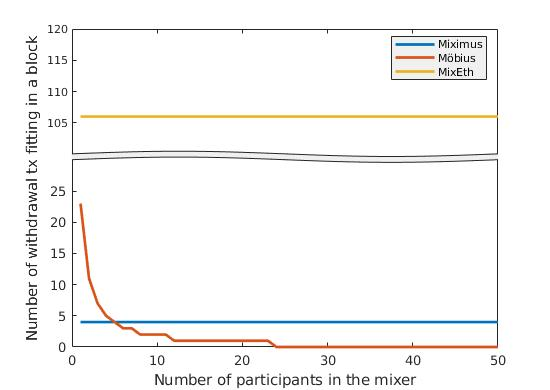
\includegraphics[scale=0.7]{./withdrawalComplexity.jpg}
	\captionsetup{justification=centering}
	\caption{Gas complexity of withdraw transactions for various trustless Ethereum coin mixers}
\end{wrapfigure}

We implemented MixEth with two different approaches. The first implementation of MixEth does not apply state channels, all the transactions are made on-chain. This could lead to unwanted gas costs as the number of corrupted shuffles increases. One of our main motivation with MixEth is to provide an efficient and scalable coin mixing protocol which uses as little blockchain resources, storage and gas, as possible. Therefore we also implement and evaluate MixEth applying state channels, namely shuffling and challenging a shuffle occurs off-chain and only deposit and withdrawal transactions happen on-chain.
Both of the implementations allow users to mix Ether or other ERC20-compatible, a popular Ethereum token standard, tokens. 

One of the main bottlenecks of coin mixing protocols is the withdrawal transactions' gas costs. A Miximus withdrawal transaction burns $\num[group-separator={,}]{1903305}$ gas, regardless of the number of participating parties. Since the block gas limit is $\num[group-separator={,}]{8000266}$ as of 2018, October 24 only 4 Miximus withdrawal transactions could fit in one Ethereum block. This is even worse for Möbius, since the gas cost for withdrawing coins from a Möbius mixer contract linearly increases with the numbers of participants.

All MixEth smart contracts were written in the Solidity language, which is currently the dominant language for developing Ethereum smart contracts. MixEth contracts are compiled using the latest version of the Solidity compiler in order to take advantage of the latest language features such as the possibility to return dynamic-sized arrays from contract functions. Note that these implementations are only proof-of-concept implementations, expect further improvements. All MixEth contracts are available online\footnote{https://github.com/seresistvanandras/MixEth}.  

\begin{table}[H] 
	\caption{Proof-of-concept implementation gas cost results. Expect further improvements. MixEthChannel refers to the implementation which leverages state channels for shuffling and challenging periods}
	\centering 
	\begin{tabular}{@{\extracolsep{6pt}}lccccc@{}} 
		
		\toprule
		\hline
		&Deployment&Deposit&\multicolumn{2}{c}{Shuffle}& Withdraw\\
		\cline{4-5}&&&Shuffle upload&Challenge\\
		\hline
		\midrule
		Möbius \cite{meiklejohn2018mobius}     &$\num[group-separator={,}]{1046027}$&$\num[group-separator={,}]{76123}$&0&0&$\num[group-separator={,}]{335714}$n   \\
		Miximus \cite{miximus2018}&$\num[group-separator={,}]{1751378}$&$\num[group-separator={,}]{732815}$&0&0 &$\num[group-separator={,}]{1903305}$  \\
		MixEth&TBD&\num[group-separator={,}]{99254}&\num[group-separator={,}]{138653}+\num[group-separator={,}]{40000}n&\num[group-separator={,}]{227563}&\num[group-separator={,}]{113265}  \\
		MixEthChannel&TBD&TBD&0&0&TBD\\
		\bottomrule
	\end{tabular}
	\label{table:securityproperties}
\end{table}   

\subsection{Fully on-chain implementation} \label{fullyonchainimpl}

\begin{wrapfigure}{r}{0.3\textwidth}
	\centering
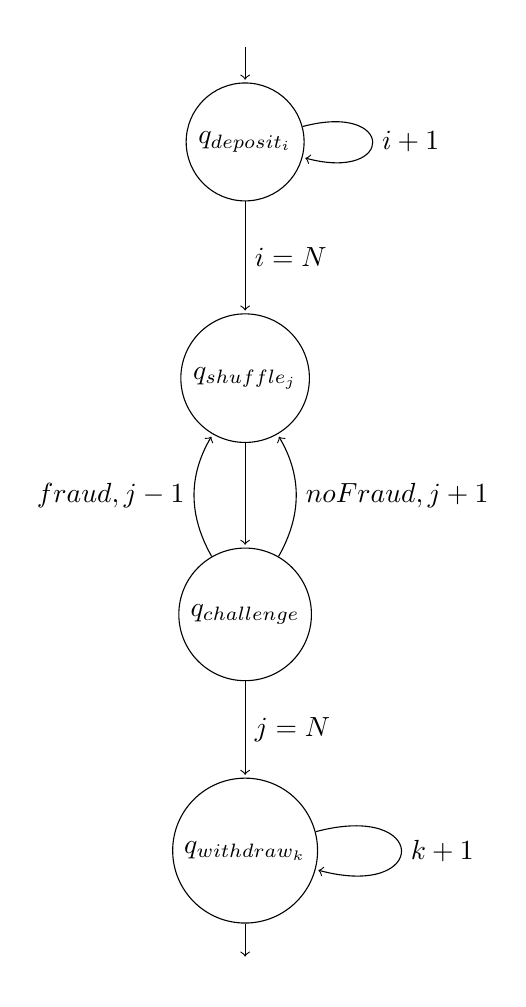
\begin{tikzpicture}[shorten >=1pt,node distance=3cm,on grid,auto] 
\node[state,initial above,initial text=] (q_deposit) {$q_{deposit_{i}}$}; 
\node[state] (q_shuffle) [below=of q_deposit ] {$q_{shuffle_{j}}$};
\node[state] (q_challenge) [below=of q_shuffle ] {$q_{challenge}$};
\node[state, accepting below, below=of q_challenge] (q_withdraw) {$q_{withdraw_{k}}$};
\path[->]
(q_deposit) edge [loop right] node {$i+1$} ()
(q_deposit) edge node {$i=N$} (q_shuffle)		
(q_shuffle) edge node {} (q_challenge)
(q_challenge) edge [bend right, swap] node {$noFraud, j+1$} (q_shuffle)
(q_challenge) edge [bend left] node {$fraud, j-1$} (q_shuffle)
(q_challenge) edge node {$j=N$} (q_withdraw)
(q_withdraw) edge [loop right] node {$k+1$} ();
\end{tikzpicture}
\captionsetup{justification=centering}
\caption{Shuffle-and-challenge paradigm implemented for the fully on-chain version of MixEth}
\end{wrapfigure}

In our first implementation of the MixEth protocol, we assumed that all transactions will take place on-chain. Since on-chain storage is extremely expensive, we decided to store only the last two sets of shuffled public keys. Note that storing only the latest shuffle would not be enough, since honest receivers could not prove to the contract that their shuffled public key is compromised unless also the last but first shuffled key is also available for the contract. Such a storage structure implies that after uploading the new shuffled keys, a challenging period should proceed in order to let receivers check the correctness of the shuffle. Furthermore we also allow senders to shuffle and deposit new public keys at the same time, meaning that only $2$ on-chain transactions are sufficient to complete the protocol. However shufflers need to withdraw their shuffling deposits with an additional on-chain transaction. We left it as a future work to determine the optimal ratio of mixed coins and shuffling deposits in order to incentivise correct shuffling.

A great advantage of the fully on-chain version of MixEth is that it allows dynamic anonymity sets. One could potentially deposit funds to the contract and shuffle public keys and leave funds in the mixing contract for indefinite amount of time. As soon as the anonymity set is large enough a receiver could withdraw their assets. This dynamic nature of the contract could even lead to a single monolithic MixEth contract instead of having multiple MixEth contracts with significantly fragmented anonymity sets. However note that the gas complexity of shuffling transactions grow linearly in the number of participants, therefore the fully on-chain implementation is not capable to support extremely large anonymity sets with participants more than cca. $300$. 

Also note that the on-chain cost of a shuffle transaction could be amortized among participants. Specifically if there is a group of senders and/or receivers who trust each other they could collectively charge any of them to shuffle once. Since they trust their peer, all the rest of the group does not need to shuffle anymore. Later non-shufflers could reimburse the only shuffler for their services either on-chain or off-chain.          

\subsection{State channel implementation} \label{statechannelimpl}

\begin{wrapfigure}{r}{0.4\textwidth}
	\centering
\begin{tikzpicture}[shorten >=1pt,node distance=4cm,on grid,auto] 
\node[state,initial above,initial text=] (q_deposit) {$q_{deposit_{i}}$}; 
\node[state] (q_shuffle) [below=of q_deposit ] {$q_{shuffle_{j}}$};
\node[state, below=of q_shuffle] (q_no_fraud) {$q_{noFraud_j}$};	\node[state, accepting, right=of q_no_fraud] (q_fraud) {$q_{fraud}$};
\node[state, accepting below, below=of q_no_fraud] (q_withdraw) {$q_{withdraw_{k}}$};
\path[->]
(q_deposit) edge [loop left] node {$i+1$} ()
(q_deposit) edge node {$i=N$} (q_shuffle)		
(q_shuffle) edge [loop left] node {$j+1$} ()
(q_shuffle) edge node {$j=N$} (q_no_fraud)
(q_no_fraud) edge node {$j=N$} (q_withdraw)
(q_no_fraud) edge [loop left] node {$j+1$} ()
(q_no_fraud) edge node {} (q_fraud)
(q_withdraw) edge [loop left] node {$k+1$} ();
\end{tikzpicture}
\captionsetup{justification=centering}
\caption{Shuffle-then-challenge paradigm implemented for the channelised version of MixEth}
\end{wrapfigure}

MixEth is also implemented in a way where shuffling and challenging periods are taking place in a state channel. We accomodated our implementation to the Counterfactual state channel framework  \cite{coleman2018counterfactual}. 

\section{Related work}
Möbius was the very first trustless coin mixer designed for Ethereum\cite{meiklejohn2018mobius}. Authors of Möbius provided formal definitions of various notions of securty such as anonymity, theft prevention and mixer availability. These properties could be used to evaluate and compare existing and future proposals from a security perspective. Möbius is a ring-signature-based trustless coin mixer with minimal on-chain transaction complexity: users of Möbius just need to create a deposit and a withdraw transaction. However the gas cost of the withdrawal transaction increases linearly in the number of receivers, which limits the size of possible anonymity sets. No more than 24 reciever could use Möbius with current cca.$\num[group-separator={,}]{8000000}$  block gas limit. If more people tries to use the mixer funds would be stucked in the mixer contract, since the gas costs of withdrawal transactions would be greater than the block gas limit. Another, maybe even more severe problem with Möbius is that withdrawal transactions can be frontrunned by anyone in the network, meaning that anyone could steal receivers' funds from the Möbius smart contract. When an honest receiver broadcasts a Möbius withdrawal transaction, other peers in the network might just create another withdrawal transaction with the very same valid linkable ring signature but with a considerably larger gas price and with their own address as recipient. Miners will act rationally and pick the transaction with the higher gas price, therefore theft-prevention in Möbius is not guaranteed.     


Miximus is a trustless zkSNARK-based mixer for Ethereum\cite{miximus2018}. It uses zkSNARKs to conceal the mapping between depositors and recipients. A depositor creates a leaf in a Merkle-tree. A depositor needs to exchange the preimage of the leaf with the recipient. Later, a recipient could prove to the Miximus contract that they know one of the preimages of a certain, undisclosed leaf. So called nullifiers enable recipients to withdraw funds once and only once. The gas costs of depositing and withdrawing funds from a Miximus mixer is independent of the number of participants. However there are disadvantages of this approach; Miximus only provides anonymity against outsiders, since if Alice funds to Bob via Miximus, Alice will know when Bob made the withdrawal transaction. Another, more severe limitation of Miximus is the trusted setup required for generating the proving key for the zkSNARK. If this trusted setup is compromised, the deployer of the contract, who generated the proving key could potentially steal funds from the mixer. Although, this issue could be amended somehow via a multi-party computation (MPC) further increasing the off-chain communication complexitiy of Miximus.

As Table \ref{table:communicationcomplexity} demonstrates, both Möbius and Miximus require $2$ on-chain transactions, while MixEth requires $3$. In spite of this seemingly added complexity, we are confident that these 3 (deposit, shuffle, withdraw) transactions consume significantly less gas than those (deposit, verify linkable ring signature/zkSNARK) of Möbius and Miximus. 
\begin{table}[H] 
\caption{Number of on-chain transactions and off-chain messages required to run a certain coin mixer protocol. Note that in case of Miximus if one wants to avoid the trusted setup for the zkSNARK, then they need to perform a secure multi-party computation protocol to trust-minimize the proving key generation.}
\centering 
\begin{tabular}{lcc} 
	
	\toprule
	&\#Off-chain messages& \#Transactions \\
	\midrule
	\textbf{Centralized} & & \\
	\midrule
	Mixcoin \cite{bonneau2014mixcoin} & 2      & 2       \\
	Blindcoin \cite{valenta2015blindcoin} & 4      & 2       \\
	TumbleBit \cite{heilman2017tumblebit} & 12      & 4      \\
	\midrule
	\textbf{Decentralized}      &    &      \\
	\midrule
	Coinjoin \cite{maxwell2013coinjoin} &  $\mathcal{O}(n^2)$     & 1       \\
	Coinshuffle \cite{ruffing2014coinshuffle} &$\mathcal{O}(n)$       & 1       \\
	XIM \cite{bissias2014sybil} & 0      & 7       \\
	Möbius \cite{meiklejohn2018mobius} & 2    & 2       \\
	Miximus \cite{miximus2018} & 1+MPC & 2 \\
	MixEth & 1 & 2 \\
	MixEthChannel  & $\mathcal{O}(n)$ &2 \\
	\bottomrule
\end{tabular}
\label{table:communicationcomplexity}
\end{table}

\section{Extensions and improvements}
MixEth is not fully compatible with the current EVM, however it could be deployed with a workaround. A recipient could ask another party or service to send a signed transaction including a signature which uses the modified version of ECDSA, where the generator element is the shuffling accumulated constant. MixEth could check this signature and send out funds to a fresh Ethereum address given in the withdraw transaction. 
 
\section{Conclusion} \label{conclusion}
 
\section{Future work}
We are going to implement and deploy MixEth on Ethereum and evaluate its performance. We are also going to give formal security proofs for the claimed security properties.  
An important and crucial research question is whether it is possible to design and implement an efficient and trustless Ethereum-based coin mixer with strong security guarantees which do not rely on any workaround and upcoming EIP implementation and is ready to be deployed on present-day Ethereum. 

\section{Acknowledgements}
We would like to thank barryWhiteHat, Dmitry Khovratovich and Sina Mahmoodi for the insightful comments and discussions. 

\bibliographystyle{plain}
\bibliography{sample}

\begin{appendices}

\section{Proof of Anonymity} \label{appendanon}
Hereby we show that if there exists an adversary $\adv$ who is able to break withdrawal anonymity defined in~\ref{sec:defanonymity}, then there exists another adversary $\bdv$ who is able to break the DDH assumption.

\begin{wrapfigure}{r}{0.5\textwidth}
	\centering
\begin{bbrenv}{A}
 \begin{bbrbox} [name=\bdv]
 \pseudocode {
 	 \text{$c_{1}\stackrel{\$}{\leftarrow}\mathbb{Z}_p$} \\
	 \text{$\textsf{PK}_{B} = (c_{0}G, c_{1}G)$} \\
	 \text{$b \stackrel{\$}{\leftarrow} \bin $} \\
	 \text{$tx \stackrel{\$}{\leftarrow}Withdraw(tumblers[j],sk_{B_{c_{b}}})$}
	 }

 \begin{bbrenv}{B}
 \begin{bbrbox}[name=\adv]
 \pseudocode{
 	 \text{Input: $PK_{B}, tx$} \\
	 \text{Output: $b^'$}
	 }
 \end{bbrbox}
 
 \end{bbrenv}
 
 \end{bbrbox}
 
 \bbrinput{$(sG,cG,c_{0}G)$}
 \bbroutput{$\lnot b\lnot{b^'}+b$}
\end{bbrenv}

\captionof{figure}{An illustration for the reduction of withdrawal anonymity to the DDH assumption}
\end{wrapfigure}

Towards contradiction let us assume that the recipient anonymity does not hold. Let us assume that the challenge to the DDH-adversary $\bdv$ is of the form $(sG,cG,c_{0}G)$. Adversary $\bdv$ generates uniformly random public key $c_{1}G$ and invokes $\adv$ with the set $\textsf{PK}_{B}=(c_{0}C^{*}, c_{1}C^{*})$, then $\bdv$ forwards $\textsf{PK}_{B}$ to $\adv$. Then a withdrawal transaction occurs from $c_{b}G$. After polynomial-time $\adv$ outputs $b^{'}$ and $\bdv$ will output $\lnot b^{'}$. If $\adv$ outputs $0$ and $b=b^{'}$, this signals to $\bdv$ that $c_{0}G$ might potentially be of the form $scG=c_{0}G$  i.e. it is a DDH tuple, therefore $\bdv$ outputs $1$. In all the other cases $\bdv$ outputs a random bit. Therefore we have that $\bdv$ has an adventage in their DDH-game if and only if $\adv$ wins their $\textsf{G}^{with, anon}_{mix, \adv}$ security game. Since we assumed that recipient anonymity does not hold we have that $$\Pr[\textsf{DDH}_{\bdv}]=\frac{1}{2}+\frac{1}{2}*\Pr[\textsf{G}^{with, anon}_{mix, \adv}]=\frac{1}{2}+\frac{1}{2}*\textsf{non-negl}(\lambda),$$ which contradicts to the DDH assumption.

\section{Proof of Availability}  \label{appendavail}
\section{Proof of Theft Prevention} \label{appendtheft}

\begin{wrapfigure}{r}{0.5\textwidth}
	\centering
	\begin{bbrenv}{A}
		\begin{bbrbox} [name=\bdv]
			\pseudocode {
				\text{$(pk_{i},sk_{i})\stackrel{\$}{\leftarrow}\kgen(1^{\lambda}) \ \forall i \in [n]$} \\
				\text{$\textsf{PK}_{B}\leftarrow\{pk_{i}\}_{i=1}^{n}$;$C, H_{\omega}, contract \leftarrow \emptyset$}
			}
			
			\begin{bbrenv}{B}
				\begin{bbrbox}[name=\adv]
					\pseudocode{
						\text{Input: $(1^{\lambda},PK_{B})$} \\
						\text{$(tx,j) \stackrel{\$}{\leftarrow}\adv^{CORR,AD,AW,HW}(1^{\lambda},PK_{B})$} \\
						\text{Output: $(tx,j)$}
					}
				\end{bbrbox}
				
			\end{bbrenv}
			
		\end{bbrbox}
		\bbrinput{$1^\lambda$}
		\bbroutput{$(tx,\sigma_{tx})$}
	\end{bbrenv}
	
	\captionof{figure}{An illustration for the reduction of theft prevention to the existentially unforgeability of ECDSA.}
\end{wrapfigure}

Towards contradiction we assume that there exists an adversary $\adv$, who is able to break the theft prevention property introduced in Section \ref{sec:theftprevention} with non-negligible probability. Using such an adversary as a subroutine we could create another efficient adversary $\bdv$ who is able to break the existential unforgeability of ECDSA. The input of the forgeability game is the security parameter which is forwarded to $\adv$ along with $n$ randomly generated public keys. By assumption $\adv$ outputs with non-negligible probability valid withdraw transaction belonging to one of the public keys in the mixer. $\bdv$ outputs the withdraw transaction and the ECDSA signature on it. $\bdv$ wins the forgeability game if and only if $\adv$ wins their $\textsf{G}^{theft}_{mix,\adv}$ game:
$$\Pr[\textsf{Forge}_{ECDSA,\bdv}]=\Pr[\textsf{G}^{theft}_{mix, \adv}]=\frac{1}{\lambda^\alpha}, $$ for some fixed $\alpha$. This contradicts to the assumption that ECDSA is existentially unforgeable.      


\end{appendices}

\end{document}
